% This is the Reed College LaTeX thesis template. Most of the work
% for the document class was done by Sam Noble (SN), as well as this
% template. Later comments etc. by Ben Salzberg (BTS). Additional
% restructuring and APA support by Jess Youngberg (JY).
% Your comments and suggestions are more than welcome; please email
% them to cus@reed.edu
%
% See https://www.reed.edu/cis/help/LaTeX/index.html for help. There are a
% great bunch of help pages there, with notes on
% getting started, bibtex, etc. Go there and read it if you're not
% already familiar with LaTeX.
%
% Any line that starts with a percent symbol is a comment.
% They won't show up in the document, and are useful for notes
% to yourself and explaining commands.
% Commenting also removes a line from the document;
% very handy for troubleshooting problems. -BTS


%%%%%%%%%%%%%%
%% Preamble %%
%%%%%%%%%%%%%%
% \documentclass{<something>} must begin each LaTeX document
\documentclass{sop_class}[overrideChapters] %modified from UF's 2019 Template --ANF
%Packages are extensions to the basic LaTeX functions. Whatever you want to
%typeset, there is probably a package out there for it. Chemistry (chemtex),
%screenplays, you name it. Check out CTAN to see: https://www.ctan.org/ Also,
%Rmarkdown can read LaTex commands in Rmd files, so long as the output is a pdf,
%because pdfs are rendered by Rmarkdown via LaTex
%%

%%amsmath, amssymb, amsthm, booktabs, caption, etoolbox, fancyhdr, flafter,
%%float, geometry, graphicx, hyperref, indentfirst, longtable, nowidow,
%%pdflscape, setspace, tabularx, threeparttablex, titlesec, titletoc,
%%and xcolor are already loaded from the 'sop_class' file

\usepackage{siunitx}
\usepackage[artemisia]{textgreek}
\usepackage[section]{placeins}
\usepackage{pdfpages}
\usepackage{calc}
\usepackage{rotating}
\usepackage{chemformula}


% Syntax highlighting #22

% So, this code uses your CSL file to decide how to format your citations
% You may need to edit your CSL if the editorial office doesn't like it
% From {rticles}
\newlength{\csllabelwidth}
\setlength{\csllabelwidth}{3em}
\newlength{\cslhangindent}
\setlength{\cslhangindent}{1.5em}
% for Pandoc 2.8 to 2.10.1
\newenvironment{cslreferences}%
  {}%
  {\par}
% For Pandoc 2.11+
% As noted by @mirh [2] is needed instead of [3] for 2.12
\newenvironment{CSLReferences}[2] % #1 hanging-ident, #2 entry spacing
 {% don't indent paragraphs
  \setlength{\parindent}{0pt}
  % turn on hanging indent if param 1 is 1
  \ifodd #1 \everypar{\setlength{\hangindent}{\cslhangindent}}\ignorespaces\fi
  % set entry spacing
  \ifnum #2 > 0
  \setlength{\parskip}{#2\baselineskip}
  \fi
 }%
 {}
\usepackage{calc} % for calculating minipage widths
\newcommand{\CSLBlock}[1]{#1\hfill\break}
\newcommand{\CSLLeftMargin}[1]{\parbox[t]{\csllabelwidth}{#1}}
\newcommand{\CSLRightInline}[1]{\parbox[t]{\linewidth - \csllabelwidth}{#1}}
\newcommand{\CSLIndent}[1]{\hspace{\cslhangindent}#1}

\providecommand{\tightlist}{%
  \setlength{\itemsep}{0pt}\setlength{\parskip}{0pt}}
% % Added by CII (Thanks, Hadley!)
% % Use ref for internal links
\renewcommand{\hyperref}[2][???]{\autoref{#1}}
\def\chapterautorefname{Chapter}
\def\sectionautorefname{Section}
\def\subsectionautorefname{Subsection}
% End of CII addition

%%%%%%%%%%%%%%%%%%%%%%%%%%%%%%%%%
% BEGIN DOCUMENT                %
%%%%%%%%%%%%%%%%%%%%%%%%%%%%%%%%%
\begin{document}

%%%%%%%%%%%%%%%%%%%%%%%%%%%%%%%%%
% TITLE PAGE                    %
%%%%%%%%%%%%%%%%%%%%%%%%%%%%%%%%%

\docBodyfalse
\begin{center}
    \thispagestyle{empty}%
      \vspace*{-0.4in}\realSingleSpace{STANDARD OPERATING PROCEDURES FOR THE MASS-REARING OF \emph{GALLERIA MELLONELLA}}%
          \vfill%
            FLORIDA DEPARTMENT OF AGRICULTURE AND CONSUMER SERVICES\\
            {Nicole ``Nikki'' Fried}, Commissioner\\
            \bigbreak%
            
            DIVISION OF \MakeUppercase{Plant Industry}\\
            {Dr.~Trevor Smith}, Director\\
            \bigbreak%
            
            BUREAU OF \MakeUppercase{Methods and Biological Control}\\
            {Dr.~Eric Rohrig}, Bureau Chief\\
            \bigbreak%
             
              % \begin{figure}[h]
              %    \includegraphics[width=0.8\textwidth]{figure/symp-rrd.png}
              % \end{figure}
            
            \vspace*{4in}%
            
            DUNDEE BIOLOGICAL CONTROL LABORATORY\\
            Dr. Austin N. Fife, Biological Scientist IV\\
            \bigbreak%
            
            Revised {September 2022}\\ 
          \vfill%
\end{center}
\newpage

%%%%%%%%%%%%%%%%%%%%%%%%%%%%%%%%%
% TABLE OF CONTENTS             %
%%%%%%%%%%%%%%%%%%%%%%%%%%%%%%%%%

\realSingleSpace
  \tableofcontents % Table of Contents comes fourth.


% %%%%%%%%%%%%%%%%%%%%%%%%%%%%%%%%%
% % LIST OF TABLES                %
% %%%%%%%%%%%%%%%%%%%%%%%%%%%%%%%%%
% %List of tables comes next, if you have one.
% \listoftables  
%   \addcontentsline{toc}{chapter}{LIST OF TABLES}
% 

%%%%%%%%%%%%%%%%%%%%%%%%%%%%%%%%%
% LIST OF FIGURES               %
%%%%%%%%%%%%%%%%%%%%%%%%%%%%%%%%%
% %List of figures comes next, if you have one.
\listoffigures
  \addcontentsline{toc}{chapter}{LIST OF FIGURES}


%%%%%%%%%%%%%%%%%%%%%%%%%%%%%%%%%
% CHAPTERS                      %
%%%%%%%%%%%%%%%%%%%%%%%%%%%%%%%%%
%TODO: get double spacing to work
\let\realSingleSpace\relax
    {\hypertarget{crw}{%
\chapter{\texorpdfstring{THE GREATER WAX MOTH, \emph{GALLERIA MELLONELLA}}{THE GREATER WAX MOTH, GALLERIA MELLONELLA}}\label{crw}}

\hypertarget{introduction}{%
\section{Introduction}\label{introduction}}
\begin{quote}
``Know your insect''

\textemdash Allen Carson Cohen
\end{quote}
moth intro

This document will continue to be updated to include the newest research relevant to the DBCL's research goals, and should be considered a work-in-progress. This SOP includes some adaptions based on the resources available at our rearing facility at the DBCL, your facility may require significant adaptations in order to fulfill your rearing needs. With that being said, these operating procedures come with no \emph{guarantee} of suitability for any particular purpose. Even so, we wish you the best of luck in your endeavors to mass-rear these beautiful invertebrates.

\newpage \clearpage

\hypertarget{moth-timeline}{%
\section{Moth Development Timeline}\label{moth-timeline}}

moths
\begin{itemize}
\tightlist
\item
  lifecycle
\end{itemize}
\hypertarget{ethics}{%
\section{ETHICAL AND HUMANE TREATMENT OF ORGANISMS}\label{ethics}}

We at the Dundee Biological Control Laboratory strongly encourage that each lab adopt a policy for the humane and ethical treatment of the organisms they work with.
\begin{enumerate}
\def\labelenumi{\arabic{enumi}.}
\tightlist
\item
  Recognizing the diversity and complexity of life systems, we value all living things
\item
  In light of this value, we try to design our work to help us understand the nature of life and living systems with a minimum of harm to or discomfort of living organisms
\item
  We treat the subjects of our studies with respect, dignity, and with efforts to inflict a minimum of pain, trauma, or damage. This includes using, whenever possible, physical models instead of living systems to conduct our experiments.
\item
  We first consider ways that can inflict a minimum of potential harm to organisms and we ask the question: is the experiment necessary to give us the information we seek? Is the information of sufficient value to merit such sacrifices?
\item
  Furthermore, we subscribe to the tenet that the information derived from studies of organisms can be no better than the health, homeostasis, and minimization of stress of the organisms involved. Therefore, we strive to make our rearing systems and every other aspect of our handling of insects compatible with insect well-being.
\end{enumerate}
Translation of these tenets into practice:
\begin{enumerate}
\def\labelenumi{\arabic{enumi}.}
\tightlist
\item
  We use the concept of insect homeostasis of ``comfort'' in the sens that sensitive and reasonable thought about our insect handling can suggest guidelines about issues like food quality, space, management of waste, access to avoidance of adverse stimuli, sufficient gas exchange, protection from contaminants and pathogens, and all other aspects of insects' well-being as it would pertain to the populations of insects in the wild
\item
  We subscribe to the model that teaches that well-treated insects are closer to ``normal'' insects from the wild. Such insects are of higher quality than ones that have been reared under suboptimal conditions. Therefore, we believe that our science is better when all aspects of our inquires are conducted with the highest possible quality of components.
\item
  Therefore, our research into development and improvement of rearing systems keeps at its forefront the homeostasis of the insects subjects in our studies, and we further strive continuously to improve the base of knowledge for the scientific community to improve the conditions of rearing systems and the quality and well-being of the subjects.
\end{enumerate}
\hypertarget{adult-cages}{%
\chapter{ADULT CAGES}\label{adult-cages}}

\hypertarget{materials}{%
\section{Materials}\label{materials}}
\begin{itemize}
\item
  Datasheets (\ref{appendix})
\item
  Insect cage
\end{itemize}
\hypertarget{methods}{%
\section{Methods}\label{methods}}

\hypertarget{insect-cages}{%
\subsection{Insect Cages}\label{insect-cages}}

Label each cage is with the following: I = date initially set, T= date
when new adults are added, and \# = current number of adults in the
cage.
\begin{itemize}
\item
  Add new `T' labels each time new adult weevils are added to a cage,
  and update the `\#' as insect populations change.
\item
  Write clearly and legibly, or print labels with a label maker to
  avoid misunderstandings.
\item
  Record all information in the appropriate datasheets found in
  \ref{appendix}.
\end{itemize}
\begin{figure}

{\centering 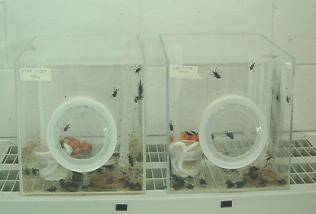
\includegraphics[width=1\linewidth]{figure/adult_cage} 

}

\caption[Cages for adult \textit{Diaprepes abbreviatus}]{Cages for adult \textit{Diaprepes abbreviatus}: One new cage is started each month with around 50 adult \textit{D. abbreviatus} per cubic foot}\label{fig:adult-cage}
\end{figure}
\hypertarget{selecting-weevils}{%
\subsection{Selecting Healthy Adult Weevils}\label{selecting-weevils}}
\begin{itemize}
\tightlist
\item
  beans
\end{itemize}
\hypertarget{art-diet-prep}{%
\chapter{WAXMOTH ARTIFICIAL DIETS}\label{art-diet-prep}}

\hypertarget{materials-1}{%
\section{Materials}\label{materials-1}}
\begin{itemize}
\tightlist
\item
  Diet ingredients, see below
\end{itemize}
\hypertarget{optimized-diet}{%
\subsection{\texorpdfstring{Optimized Diet for \emph{Galleria mellonella}}{Optimized Diet for Galleria mellonella}}\label{optimized-diet}}
\begin{longtable}[]{@{}llll@{}}
\caption{From Hickin et al. (\protect\hyperlink{ref-Hickin2021}{2021}).}\tabularnewline
\toprule()
Ingredient & Amount & Unit & Percentage of diet \\
\midrule()
\endfirsthead
\toprule()
Ingredient & Amount & Unit & Percentage of diet \\
\midrule()
\endhead
Oat bran & 14 & grams & 4.9\% \\
Wheat bran & 34 & grams & 12.0\% \\
Rice bran & 20 & grams & 7.1\% \\
Torula yeast & 42 & grams & 14.8\% \\
Beeswax & 11 & grams & 3.9\% \\
Honey & 68 & grams & 24.0\% \\
Glycerol & 64 & grams & 22.6\% \\
Deionized water & 30 & milliliters & 10.6\% \\
\bottomrule()
\end{longtable}
This is the preferred diet used for mass-rearing \emph{Galleria mellonella.}

\clearpage
\newpage

\hypertarget{old-diet}{%
\subsection{Historical Artificial Diet}\label{old-diet}}
\begin{longtable}[]{@{}lll@{}}
\caption{For reference only, not recommended for use in mass-rearing.}\tabularnewline
\toprule()
Ingredient & Amount & Unit \\
\midrule()
\endfirsthead
\toprule()
Ingredient & Amount & Unit \\
\midrule()
\endhead
Cellulose & 307 & grams \\
\bottomrule()
\end{longtable}
\hypertarget{methods-1}{%
\section{Methods}\label{methods-1}}

\hypertarget{pre-sanitation}{%
\subsection{Sanitation Before Making Artificial Diet}\label{pre-sanitation}}

beans

\hypertarget{diet-prep}{%
\subsection{Diet Preparation Instructions}\label{diet-prep}}

\hypertarget{paper-strips}{%
\chapter{OVIPOSITION STRIPS AND EGG COLLECTION}\label{paper-strips}}

\hypertarget{materials-2}{%
\section{Materials}\label{materials-2}}
\begin{itemize}
\tightlist
\item
  Wax or butcher paper
\end{itemize}
\hypertarget{methods-2}{%
\section{Methods}\label{methods-2}}

\hypertarget{baggie-prep}{%
\subsection{Preparing Storage Bags}\label{baggie-prep}}

Collect egg strips daily at the beginning of the day to avoid cross

\hypertarget{neonate-transfer}{%
\chapter{TRANSFERRING NEONATE LARVAE}\label{neonate-transfer}}

\hypertarget{materials-3}{%
\section{Materials}\label{materials-3}}
\begin{itemize}
\tightlist
\item
  Büchner funnel
\item
  Fast flow filter paper
\end{itemize}
\hypertarget{methods-3}{%
\section{Methods}\label{methods-3}}

\hypertarget{make-grub-shake}{%
\subsection{Creating a Grub Shaker}\label{make-grub-shake}}

Transferring newly hatched

\hypertarget{sterilizing-neonates}{%
\subsection{Surface Sterilizing Neonate Larvae}\label{sterilizing-neonates}}

Any fungal spores or bacteria on the skin of the larvae will be
transferred directly to the diet cups, so it is necessary to sterilize
the larvae before they are transferred to avoid contamination.
Transferring larvae should be done in a clean room on a sanitized
surface, while wearing surgical gloves, facemasks, and hairnets to
reduce the risks of microbial contamination.
\begin{enumerate}
\def\labelenumi{\arabic{enumi}.}
\tightlist
\item
  Sanitize any surfaces and utensils which will be used by spraying
  and wiping the work space with 75\% isopropyl alcohol.
\end{enumerate}
\hypertarget{moth-transfers}{%
\chapter{TRANSFERRING MOTHS}\label{moth-transfers}}

\hypertarget{materials-4}{%
\section{Materials}\label{materials-4}}
\begin{itemize}
\tightlist
\item
  Forceps
\item
  Soft forceps
\end{itemize}
\hypertarget{methods-4}{%
\section{Methods}\label{methods-4}}

The original diet cups become overcrowded around 4 weeks (\textasciitilde28 days) as
the larvae grow.

\hypertarget{sanitizing-and-preparing-grubs-for-transfer}{%
\subsection{Sanitizing and Preparing Grubs for Transfer}\label{sanitizing-and-preparing-grubs-for-transfer}}
\begin{enumerate}
\def\labelenumi{\arabic{enumi}.}
\tightlist
\item
  Cups contaminated with bacteria or mold should be removed prior to
  separation of grubs and recorded as losses on the \emph{Galleria}
  discard datasheet, \ref{discard-datasheet}.
\end{enumerate}
\hypertarget{shipping}{%
\chapter{SHIPPING}\label{shipping}}

\textbf{Ship overnight on the sender's account number for institutions
(Universities, USDA, researchers, etc.) and on our own account number
for civilians. Include a return label as necessary. Remember to include a copy of our permit when shipping pests like \textit{Diaprepes!}}

\hypertarget{ship-larvae-pupae}{%
\section{Larvae and Pupae}\label{ship-larvae-pupae}}

Larvae and Pupae can be shipped in 50 ml centrifuge tubes with diet.
\begin{enumerate}
\def\labelenumi{\arabic{enumi}.}
\item
  Place cups with diet and larvae in 50 ml centrifuge tube trays and place 2
  trays in a large Ziploc®-style plastic freezer baggie.
\item
  Put bagged trays together in a larger bag or trash bag.
\item
  Put in appropriate size box, fill space with bubble wrap or air
  bags, etc.
\item
  Tape box well, reinforce the bottom of the box with tape.
\item
  Label with `This side up' before shipping.
\end{enumerate}
\hypertarget{ship-adults}{%
\section{Adults}\label{ship-adults}}

Teneral adults in their diet cups can be shipped as-is, in the same way
we ship larvae.
\begin{enumerate}
\def\labelenumi{\arabic{enumi}.}
\item
  Adults from cages can be shipped in an empty clean diet cup with a
  damp dental wick.
\item
  Ship with a ice pack wrapped a paper towel.
\item
  Do not use an ice pack for teneral adults.
\end{enumerate}
\hypertarget{ship-eggs}{%
\section{Eggs}\label{ship-eggs}}

Eggs are more fragile, but can still be shipped if needed.
\begin{enumerate}
\def\labelenumi{\arabic{enumi}.}
\item
  If shipping eggs, ship freshly laid eggs, eggs about to hatch do not
  survive well.
\item
  Double-bag eggs in small to medium ziploc baggies with the air
  gently squeezed out from the bag to prevent desiccation.
\item
  \textbf{Be careful not to squash eggs when squeezing out air!}
\item
  Ensure both zippers on the plastic baggie are sealed well.
\item
  Place the nested baggies into a large bag inflated with air, to help
  protect eggs from damage.
\item
  Pack the baggies in a small box with plenty of bubble wrap or air
  bags.
\end{enumerate}
\hypertarget{facility}{%
\chapter{SANITATION AND MAINTENANCE}\label{facility}}

\hypertarget{materials-5}{%
\section{Materials}\label{materials-5}}
\begin{itemize}
\tightlist
\item
  beans
\end{itemize}
\hypertarget{methods-5}{%
\section{Methods}\label{methods-5}}
\begin{itemize}
\tightlist
\item
  beans
\end{itemize}
\hypertarget{daily-duties}{%
\section{Daily Duties}\label{daily-duties}}
\begin{itemize}
\tightlist
\item
  Sinks: Wash dishes using a mild detergent and rinse with 37.5 mls of
  bleach per gallon of water. Empty and rinse sinks in all rooms at
  end of day.
\item
  Garbage: Remove garbage and place in freezer for 24 hour duration,
  after which the material is taken to the dumpster.
\item
  Counters and Table Tops: Spray surfaces with 10\% bleach at the
  beginning and end of work schedule.
\item
  Floors: Sweep and Mop with bleach
\end{itemize}
\hypertarget{weekly-duties}{%
\section{Weekly Duties}\label{weekly-duties}}
\begin{itemize}
\tightlist
\item
  Floors: Sweep all rooms (Q.C. 1,2,and 3), and mop with detergent and
  water.
\end{itemize}
\hypertarget{monthly-duties}{%
\section{Monthly Duties}\label{monthly-duties}}
\begin{itemize}
\tightlist
\item
  Apply standard quaternary ammonia solution to ceilings, cupboards
  and drawers, lights, walls and doors using swivel head mop to the
  following surfaces in Q.C. 1, 2, and 3.
\item
  AC vents: Remove from the ceiling and spray with water, followed by
  application of the standard solution of quaternary ammonia.
\end{itemize}
As the above sanitation duties are completed, it is recorded on the
Sanitation Checklist Form, SFL 01-10 (see Appendix A-7).

\hypertarget{rearing-organization}{%
\section{Rearing Area Organization}\label{rearing-organization}}

Persistence of contamination in lab reared insect colonies has led to
separation of colony stages.
\begin{itemize}
\item
  Q.C. 1, has been designated a ``dirty area'' and as such is reserved
  for the adult egg laying cages and contaminated cultures held for
  recovery.
\item
  Q.C. 2, has been designated ``semi clean'', and is reserved for
  cultures 30 days or older (neonate larvae which have been
  transferred to single cups, and later stages of the life cycle
  including pupae and teneral adults).
\item
  Q.C. 3, has been designated ``clean'', and as such is reserved for new
  cultures only, and these cultures should be moved to Q.C. 2 at the
  time of transfer.
\end{itemize}
\hypertarget{order-of-duties}{%
\section{Order of Duties}\label{order-of-duties}}

Organization and order of duties are directly related.
\begin{itemize}
\item
  Clean work should be performed in the morning prior to exposure of
  equipment/ personnel to contaminants.
\item
  Duties such as neonate transfers and sanitation of Q.C. 3 fall into
  this category.
\item
  Semi-clean work should be performed next.
\item
  This includes separation of neonate larvae, transfers to fresh diet,
  and sanitation of Q.C. 2.
\item
  Dirty work should be performed last.
\item
  This includes egg collection, cage maintenance, and sanitation of
  Q.C. 1.
\item
  Moving from dirty areas to clean ones should be avoided.
\item
  It is important to keep in mind where you have been, and what has
  been handled.
\end{itemize}
\hypertarget{supply-inventory}{%
\section{Supply Inventory}\label{supply-inventory}}

Supplies should be checked periodically to ensure that shortages do not
occur.

A list of needed items should be given to the immediate supervisor or
purchaser, based on lead time necessary to obtain these items. (See
Appendix A-1 for suppliers.)

\hypertarget{cleaning-used-mats}{%
\subsection{Disposal and Cleaning Used Materials}\label{cleaning-used-mats}}

\hypertarget{dispose-flush}{%
\subsubsection{Disposal of flush removed from cage}\label{dispose-flush}}
\begin{enumerate}
\def\labelenumi{\arabic{enumi}.}
\item
  Dispose of in trash bags and take to the steamer, or freeze prior to
  putting in dumpster.
\item
  Collect dirty vials, water cups, etc. and take to A105.
\item
  Wash vials and water cups and lids with dawn dish detergent and
  scrub with bottle brushes OR rinse and put in a dishpan with
  detergent to soak; then wash later.
\end{enumerate}
\hypertarget{dispose-water}{%
\subsubsection{Disposal of water cups}\label{dispose-water}}
\begin{enumerate}
\def\labelenumi{\arabic{enumi}.}
\item
  Prior to washing water cups, remove cotton wicks, do not get
  detergent on water wicks, can rinse with clean water, and gently
  brush with small bottle brush.
\item
  Can reuse until they become soiled to the point that the above
  cleaning methods are no longer effective.
\end{enumerate}
\hypertarget{materials-6}{%
\section{Materials}\label{materials-6}}
\begin{itemize}
\tightlist
\item
  Parafilm®
\end{itemize}
\hypertarget{potato-dextrose-agar}{%
\subsection{Potato Dextrose Agar}\label{potato-dextrose-agar}}
\begin{longtable}[]{@{}lll@{}}
\caption{For culturing fungi. (\protect\hyperlink{ref-FDA2020}{FDA 2020}, \protect\hyperlink{ref-FDA2022}{2022})}\tabularnewline
\toprule()
Ingredient & Amount & Unit \\
\midrule()
\endfirsthead
\toprule()
Ingredient & Amount & Unit \\
\midrule()
\endhead
Potato Infusion & 200 & grams \\
Dextrose & 20 & grams \\
Agar & 20 & grams \\
Sodium Chloride* & 75 & grams \\
Deionized water & 1000 & milliliters \\
Chlortetracycline-HCl (stock solution)** & 4 & milliliters \\
\bottomrule()
\end{longtable}
*Optional. Used to to make Potato Dextrose Salt Agar (PDS-A). Cultures
fungi with spreading habits, such as \emph{Mucor}, \emph{Rhizopus}, and similar
fungi (\protect\hyperlink{ref-Mislivec1991}{Mislivec and Stack 1991}). **Optional. See \ref{pda-antibio} and
Mislivec and Stack (\protect\hyperlink{ref-Mislivec1991}{1991}).

\hypertarget{nutrient-agar}{%
\subsection{Nutrient Agar}\label{nutrient-agar}}
\begin{longtable}[]{@{}lll@{}}
\caption{For culturing bacteria. (\protect\hyperlink{ref-FDA2020}{FDA 2020}, \protect\hyperlink{ref-FDA2022}{2022}).}\tabularnewline
\toprule()
Ingredient & Amount & Unit \\
\midrule()
\endfirsthead
\toprule()
Ingredient & Amount & Unit \\
\midrule()
\endhead
Beef extract & 3 & grams \\
Peptone & 5 & grams \\
Agar & 15 & grams \\
Deionized water & 1000 & milliliters \\
\bottomrule()
\end{longtable}
\hypertarget{methods-6}{%
\section{Methods}\label{methods-6}}

\hypertarget{environmental-microbiology}{%
\subsection{Testing for Environmental Contaminants}\label{environmental-microbiology}}

Follow the sanitation programs as described in \ref{facility} and
\ref{sanitation-checklist} to prevent contamination of \emph{Galleria}
cultures. Monitor the levels of microbial contaminants weekly by `air
plating' agarose petri dishes to detect the relative quantities of mold,
bacteria, and yeast present. Monitoring for microbial contaminants helps
to ensure that the sanitation programs are effective and to make sure
areas are adequately sterilized. The goal of sampling air quality is to
quantify the number of particles of contaminant in the air, usually
expressed in terms of the colony forming units (CFUs) per cubic meter of
sampled air during a specific time period (CFU/m\(^3\)/time)
(\protect\hyperlink{ref-Romano2015}{Romano 2015}).

Our lab uses two types of enriched agarose media to culture and detect
contaminants: Potato Dextrose Agar (PDA) and Nutrient Agar, for fungi
and bacteria, respectively.

\hypertarget{prep-media}{%
\subsection{Preparing Agarose Media}\label{prep-media}}

\hypertarget{nutri-agar}{%
\subsubsection{Nutrient Agar}\label{nutri-agar}}
\begin{itemize}
\item
  Mix dry ingredients, then add to 1 L of DI water.
\item
  Heat to boiling while stirring until ingredients are dissolved.
\item
  Dispense into petri dishes.
\item
  Once all the ingredients are completely dissolved, pour into
  containers that can be autoclaved and autoclave for 15 min at 121
  °C.
\item
  Dispense 20-25 ml portions into sterile 15 × 100 mm petri dishes.
\item
  Adjust final pH as needed to be 6.8 ± 0.2.
\end{itemize}
\hypertarget{make-up-pda}{%
\subsubsection{Potato Dextrose Agar (PDA)}\label{make-up-pda}}

PDA medium powder is available commercially but you may need to add
extra agar until there is a total of 20 g/liter of agar in the final
product. For example, you would need to add 5 g of agar to BBL™ or
Difco™ dehydrated medium to have a plate with the correct consistency.
PDA medium should not be re-melted more than once.
\begin{enumerate}
\def\labelenumi{\arabic{enumi}.}
\tightlist
\item
  Create potato infusion by boiling 200 g of sliced, unpeeled potatoes
  in 1 L DI water for 30 mins.
\item
  Filter solution through cheesecloth and retain the liquid, which is
  potato infusion. Alternatively, purchase dehydrated potato infusion
  and prepare according to the manufacturer's instructions.
\item
  Mix in 20 g Dextrose and 20 g Agar with the 1 L of potato infusion,
  then stir while bringing to a boil to dissolve the agar.
\item
  Once all the ingredients are completely dissolved, pour into
  containers that can be autoclaved and autoclave for 15 min at 121
  °C.
\item
  Dispense 20-25 ml portions into sterile 15 × 100 mm petri dishes.
\item
  Adjust final pH as needed to be 5.6 ± 0.2 pH.
\end{enumerate}
\hypertarget{pda-antibio}{%
\subsubsection{Preventing bacterial growth in PDA media}\label{pda-antibio}}

We want to focus on the fungi present in the PDA media, so if bacterial
contamination becomes a problem, we can add an antibiotic to the media
to avoid this issue. Mislivec and Stack (\protect\hyperlink{ref-Mislivec1991}{1991}) mentions their preference for
Chlortetracycline-HCl, but suggests that other antibiotics such as
chloramphenicol or streptomycin can be used in addition to
chlortetracycline-HCl. If adding an additional antibiotic, use the same
concentration as the chlortetracycline-HCl (40 ppm).
\begin{enumerate}
\def\labelenumi{\arabic{enumi}.}
\tightlist
\item
  Prepare a stock solution of Chlortetracycline-HCl by dissolving 19 g
  of antibiotic in 100 ml of sterilized DI water
\item
  Filter stock solution through a 0.45 µm membrane (Nalge Sybron
  Corp., Rochester, NY). and pour into an aluminum-wrapped amber
  bottle.
\item
  Store stock solutions in the dark at 4-8 °C. A properly stored
  solution should last for at least a month.
\item
  Allow stock solutions to reach room temperature immediately before
  use.
\item
  PPM calculation: add 1 ml of 100 ml stock solution for every 250 ml
  of media to obtain a concentration of 40 ppm.
\item
  Add Chlortetracycline-HCl to PDA media at a rate of 40 ppm (final
  concentration) after agar has been autoclaved and cooled to 47-50
  °C.
\item
  Mix thoroughly and dispense 20 ml portions into 15 × 100 mm petri
  dishes.
\item
  Dispense 4 ml of stock filter-sterilized chlortetracycline HCl (1
  g/100 ml) per liter of agarose medium.
\end{enumerate}
\hypertarget{gravity-testing}{%
\subsection{Sedimentation Plates}\label{gravity-testing}}

An inexpensive and simple method of sampling for aerial microbes is with
sedimentation plates, aka. settling plates. Sedimentation plates rely on
gravity to cause airborne particles to land on the exposed surface of
petri dishes filled with agarose media. These plates are then incubated
for 48 hours and the number of CFUs are counted. Viable particles will
grow into CFUs, which then can be counted to quantify the level of
contamination in the area. In practice sedimentation plates have a bias
towards larger particles, and tend to underestimate the number of
smaller particles (\protect\hyperlink{ref-Bourdillon1941}{Bourdillon et al. 1941}, \protect\hyperlink{ref-Schneider2009}{Schneider 2009}). Due to these
shortcomings, the use of sedimentation plates should be used as a
preliminary assay only.

\hypertarget{sedimentation-plates}{%
\subsubsection{Sedimentation plate assays}\label{sedimentation-plates}}
\begin{enumerate}
\def\labelenumi{\arabic{enumi}.}
\tightlist
\item
  Leave a petri dish of PDA and a dish of NA uncovered for 1 hour in
  each area where insects or diet are handled. More plates can be
  added for larger areas, or for specific point samples.
\item
  Replace lid of petri dish, and wrap the edges of the dish with
  Parafilm®
\item
  Incubate plates in lab oven at 30 °C
\item
  Incubate for 2 days (48 hours) for NA media, and 4 days (96 hours)
  for PDA media.
\item
  Record the number and type of microorganisms on the Environmental
  Testing Datasheet (@ref()) .
\end{enumerate}
\docBodyfalse
\setcounter{secnumdepth}{-1}

\realSingleSpace

\hypertarget{references}{%
\chapter*{REFERENCES}\label{references}}
\addcontentsline{toc}{chapter}{REFERENCES}

\hypertarget{refs}{}
\begin{CSLReferences}{1}{1}
\leavevmode\vadjust pre{\hypertarget{ref-Bourdillon1941}{}}%
\textbf{Bourdillon, R. B., O. M. Lidwell, and J. C. Thomas}. \textbf{1941}. A slit sampler for collecting and counting air-borne bacteria. Epidemiology \& Infection. 41: 197--224, DOI:\href{https://doi.org/10.1017/S0022172400012407}{10.1017/S0022172400012407}.

\leavevmode\vadjust pre{\hypertarget{ref-FDA2020}{}}%
\textbf{FDA}. \textbf{2020}. \href{https://www.fda.gov/food/laboratory-methods-food/bam-media-m127-potato-dextrose-agar}{BAM Media M127: Potato Dextrose Agar}. Food; Drug Administration Center for Food Safety; Applied Nutrition.

\leavevmode\vadjust pre{\hypertarget{ref-FDA2022}{}}%
\textbf{FDA}. \textbf{2022}. \href{https://www.fda.gov/food/laboratory-methods-food/bacteriological-analytical-manual-bam}{Bacteriological Analytical Manual (BAM)}, 8th ed. Food; Drug Administration Center for Food Safety; Applied Nutrition.

\leavevmode\vadjust pre{\hypertarget{ref-Hickin2021}{}}%
\textbf{Hickin, M., H. Nadel, C. Schal, and A. C. Cohen}. \textbf{2021}. Optimization of a diet for the greater wax moth (lepidoptera: Pyralidae) using full factorial and mixture design. Journal of Economic Entomology. 114: 1091--1103, DOI:\href{https://doi.org/10.1093/jee/toab039}{10.1093/jee/toab039}.

\leavevmode\vadjust pre{\hypertarget{ref-Mislivec1991}{}}%
\textbf{Mislivec, P., and M. E. Stack}. \textbf{1991}. \href{https://www.fao.org/3/x5036e/x5036E0o.htm}{Enumeration of yeasts and moulds and production of toxins}. \emph{In} Semple, R.L., Frio, A.S., Hicks, P.A., Lozare, J.V. (eds.),. UNDP/FAO Regional Network Inter-Country Cooperation on Postharvest Technology; Quality Control of Foodgrains, Bangkok, Thailand.

\leavevmode\vadjust pre{\hypertarget{ref-Schneider2009}{}}%
\textbf{(Principles and procedures for rearing high quality insects) }. \textbf{2009}. Principles and procedures for rearing high quality insects. Mississippi State University, Mississippi State, MS.

\leavevmode\vadjust pre{\hypertarget{ref-Romano2015}{}}%
\textbf{Romano, F.} \textbf{2015}. Some aspects on the sampling efficiency of microbial impaction air samplers. 4, DOI:\href{https://doi.org/10.1016/j.partic.2014.11.008}{10.1016/j.partic.2014.11.008}.

\end{CSLReferences}
\docBodyfalse

\hypertarget{appendix}{%
\chapter*{APPENDIX}\label{appendix}}
\addcontentsline{toc}{chapter}{APPENDIX}

\hypertarget{source-directory}{%
\section{\texorpdfstring{SOURCE DIRECTORY FOR \emph{GALLERIA} MATERIALS}{SOURCE DIRECTORY FOR GALLERIA MATERIALS}}\label{source-directory}}

1oz Cups 1oz Cup Lids 1. Heritage Paper 822 N.W. 107 terr. Gainesville,
FL 32606 (352-332-1417) 10.75'' x 13'' Plastic food container lids 1.
Merton Restaurant Supplies. 207 W. Gore St.~Orlando, FL 32806
(407-425-4557) Citrus Root Weevil Premix 30 Cup Plastic Trays 1.
Bioserve. P.O. Box 450 Frenchtown, NJ 08825 (908-996-2155) Benzoic Acid
Methyl Paraben 3.5'', 5'' Petri Dishes 1. Fisher Scientific. 3970 Johns
Creek ct. ste. 500 Suwannee, GA 30024 (1-800-766-7000) Agar 1. Coll-Chem
Corp.~P.O. Box 721 Ridgewood, NJ 07451 (201-445-6662) Zipper Top Bags
(all sizes) Mineral Oil Organic Carrots Dawn Dish Soap Wax Paper 1.
Publix. 125 S.W. 34th st. Gainesville, FL 32607 Bleach 1.Home Depot P.O.
Box 9903 Macon, GA 31297-9903 Dental Wicks 1. Richmond Dental. P.O. Box
34276 Charlotte, NC 28234 (1-800-277-0377)

\hypertarget{diaprepes-rearing-supplies-and-sources}{%
\subsection{DIAPREPES REARING SUPPLIES AND SOURCES:}\label{diaprepes-rearing-supplies-and-sources}}

Product Product \# Source Link Dental Wick 200404 Richmond Dental
Wrapped Rolls \textbar{} Richmond Dental

24''x24''x24'' Lumite Cage 1450DS BioQuip Search (bioquip.com) 1 oz (30 ml)
clear portion containers (cups) Dart/Conex 100pc Webstaurant Store
\url{https://www.webstaurantstore.com/dart-conex-complements-100pc-1-oz-translucent-plastic-souffle-portion-cup-case/301100PC.html}
clear plastic lids for 100 PC cups PL100N Webstaurant Store
\url{https://www.webstaurantstore.com/dart-solo-pl100n-small-clear-plastic-souffle-cup-lid-case/301PL100N.html}
Pre-mix for Diaprepes Root Weevil F9855 Frontier Scientific Services
\href{mailto:sales@insectrearing.com}{\nolinkurl{sales@insectrearing.com}} +1
302-533-3540 *Special order by request Agar 7060 Frontier Scientific
Services \url{https://insectrearing.com/product/product-7060-agar/} Cup
Trays -- 30 well 9040 Frontier Scientific Services Cup Tray-30 Wells
(9040) - Frontier Scientific Services Agriculture (insectrearing.com)

\clearpage
\begin{landscape} %landscape page
\section{\textit{DIAPREPES} EGGS AND NEONATE PRODUCTION DATASHEET}\label{egg-neo-datasheet}
\begin{table}[!htbp]
    \centering
    \setlength{\tabcolsep}{0.5em}
      \begin{threeparttable}
        \rowcolors{2}{gray!10}{gray!40}
              \begin{tabular}{|c|c|c|c|c|c|c|}
            \toprule
            {Cage ID} & {EC Week (Gen)} & {No. Eggs} & {No. Clusters} & {Infest Date} & {No. Larvae} & {No. Cups}\\
            \hline
            {} & {} & {} & {} & {} & {} & {}\\
            \hline
            {} & {} & {} & {} & {} & {} & {}\\
            \hline
            {} & {} & {} & {} & {} & {} & {}\\
            \hline
            {} & {} & {} & {} & {} & {} & {}\\
            \hline
            {} & {} & {} & {} & {} & {} & {}\\
            \hline
            {} & {} & {} & {} & {} & {} & {}\\
            \hline
            {} & {} & {} & {} & {} & {} & {}\\
            \hline
            {} & {} & {} & {} & {} & {} & {}\\
            \hline
            {} & {} & {} & {} & {} & {} & {}\\
            \hline
            {} & {} & {} & {} & {} & {} & {}\\
            \hline
            {} & {} & {} & {} & {} & {} & {}\\
            \hline
            {} & {} & {} & {} & {} & {} & {}\\
            \hline
            {} & {} & {} & {} & {} & {} & {}\\
            \hline
            {} & {} & {} & {} & {} & {} & {}\\
            \hline
            {} & {} & {} & {} & {} & {} & {}\\
            \hline
            {} & {} & {} & {} & {} & {} & {}\\
            \hline
            {} & {} & {} & {} & {} & {} & {}\\
            \hline
            {} & {} & {} & {} & {} & {} & {}\\
            \hline
            {} & {} & {} & {} & {} & {} & {}\\
            \hline
            {} & {} & {} & {} & {} & {} & {}\\
            \hline
            {} & {} & {} & {} & {} & {} & {}\\
            \hline
            {} & {} & {} & {} & {} & {} & {}\\
            \hline
            {} & {} & {} & {} & {} & {} & {}\\
            \hline
            \bottomrule
            \end{tabular}
        \begin{tablenotes}
            \small
            \item COMMENTS: \hfill{} rev. 09.02.2022 \\
            \\
            \\
            \\
        \end{tablenotes}
    \end{threeparttable}
\end{table}
 \end{landscape}
\begin{landscape} %landscape page
\section{\textit{DIAPREPES} GRUB, PUPAE AND ADULT PRODUCTION DATASHEET}\label{grub-adult-datasheet}
\begin{table}[!htbp]
    \centering
    \setlength{\tabcolsep}{0.5em}
      \begin{threeparttable}
        \rowcolors{2}{gray!10}{gray!40}
              \begin{tabular}{|c|c|c|c|c|c|c|c|c|}
            \toprule
            {Cage ID} & {EC Week (Gen)} & {Transfer Date} & {No. Grubs} & {Pupation Date} & {No. Pupae} & {Emerge Date} & {No. Adults} & {No. to Cages}\\
            \hline
            {} & {} & {} & {} & {} & {} & {} & {} & {}\\
            \hline
            {} & {} & {} & {} & {} & {} & {} & {} & {}\\
            \hline
            {} & {} & {} & {} & {} & {} & {} & {} & {}\\
            \hline
            {} & {} & {} & {} & {} & {} & {} & {} & {}\\
            \hline
            {} & {} & {} & {} & {} & {} & {} & {} & {}\\
            \hline
            {} & {} & {} & {} & {} & {} & {} & {} & {}\\
            \hline
            {} & {} & {} & {} & {} & {} & {} & {} & {}\\
            \hline
            {} & {} & {} & {} & {} & {} & {} & {} & {}\\
            \hline
            {} & {} & {} & {} & {} & {} & {} & {} & {}\\
            \hline
            {} & {} & {} & {} & {} & {} & {} & {} & {}\\
            \hline
            {} & {} & {} & {} & {} & {} & {} & {} & {}\\
            \hline
            {} & {} & {} & {} & {} & {} & {} & {} & {}\\
            \hline
            {} & {} & {} & {} & {} & {} & {} & {} & {}\\
            \hline
            {} & {} & {} & {} & {} & {} & {} & {} & {}\\
            \hline
            {} & {} & {} & {} & {} & {} & {} & {} & {}\\
            \hline
            {} & {} & {} & {} & {} & {} & {} & {} & {}\\
            \hline
            {} & {} & {} & {} & {} & {} & {} & {} & {}\\
            \hline
            {} & {} & {} & {} & {} & {} & {} & {} & {}\\
            \hline
            {} & {} & {} & {} & {} & {} & {} & {} & {}\\
            \hline
            {} & {} & {} & {} & {} & {} & {} & {} & {}\\
            \hline
            {} & {} & {} & {} & {} & {} & {} & {} & {}\\
            \hline
            {} & {} & {} & {} & {} & {} & {} & {} & {}\\
            \hline
            {} & {} & {} & {} & {} & {} & {} & {} & {}\\
            \hline
            \bottomrule
            \end{tabular}
        \begin{tablenotes}
            \small
            \item COMMENTS: \hfill{} rev. 09.02.2022 \\
            \\
            \\
            \\
        \end{tablenotes}
    \end{threeparttable}
\end{table}
 \end{landscape}
\clearpage
\newpage
\begin{landscape} %landscape page
\section{\textit{DIAPREPES} DISCARD DATASHEET}\label{discard-datasheet}
\begin{table}[!htbp]
    \centering
    \setlength{\tabcolsep}{0.5em}
      \begin{threeparttable}
        \caption*{Month$\colon$}
        \rowcolors{2}{gray!10}{gray!40}
              \begin{tabular}{|c|c|c|c|c|c|c|c|c|c|c|c|c|c|}
            \toprule
            \hline
            {Generation} & {Date} & {No. Cups} & {L} & {G} & {P} & {A} & {Mold} & {Mites} & {Bacteria} & {Dead} & {Slow} & {Elytra} & {Other}\\
            \hline
            {} & {} & {} & {} & {} & {} & {} & {} & {} & {} & {} & {} & {} & {}\\
            \hline
            {} & {} & {} & {} & {} & {} & {} & {} & {} & {} & {} & {} & {} & {}\\
            \hline
            {} & {} & {} & {} & {} & {} & {} & {} & {} & {} & {} & {} & {} & {}\\
            \hline
            {} & {} & {} & {} & {} & {} & {} & {} & {} & {} & {} & {} & {} & {}\\
            \hline
            {} & {} & {} & {} & {} & {} & {} & {} & {} & {} & {} & {} & {} & {}\\
            \hline
            {} & {} & {} & {} & {} & {} & {} & {} & {} & {} & {} & {} & {} & {}\\
            \hline
            {} & {} & {} & {} & {} & {} & {} & {} & {} & {} & {} & {} & {} & {}\\
            \hline
            {} & {} & {} & {} & {} & {} & {} & {} & {} & {} & {} & {} & {} & {}\\
            \hline
            {} & {} & {} & {} & {} & {} & {} & {} & {} & {} & {} & {} & {} & {}\\
            \hline
            {} & {} & {} & {} & {} & {} & {} & {} & {} & {} & {} & {} & {} & {}\\
            \hline
            {} & {} & {} & {} & {} & {} & {} & {} & {} & {} & {} & {} & {} & {}\\
            \hline
            {} & {} & {} & {} & {} & {} & {} & {} & {} & {} & {} & {} & {} & {}\\
            \hline
            {} & {} & {} & {} & {} & {} & {} & {} & {} & {} & {} & {} & {} & {}\\
            \hline
            {} & {} & {} & {} & {} & {} & {} & {} & {} & {} & {} & {} & {} & {}\\
            \hline
            {} & {} & {} & {} & {} & {} & {} & {} & {} & {} & {} & {} & {} & {}\\
            \hline
            {} & {} & {} & {} & {} & {} & {} & {} & {} & {} & {} & {} & {} & {}\\
            \hline
            {} & {} & {} & {} & {} & {} & {} & {} & {} & {} & {} & {} & {} & {}\\
            \hline
            {} & {} & {} & {} & {} & {} & {} & {} & {} & {} & {} & {} & {} & {}\\
            \hline
            {} & {} & {} & {} & {} & {} & {} & {} & {} & {} & {} & {} & {} & {}\\
            \hline
            {} & {} & {} & {} & {} & {} & {} & {} & {} & {} & {} & {} & {} & {}\\
            \hline
            {} & {} & {} & {} & {} & {} & {} & {} & {} & {} & {} & {} & {} & {}\\
            \hline
            {} & {} & {} & {} & {} & {} & {} & {} & {} & {} & {} & {} & {} & {}\\
            \hline
            \bottomrule
            \end{tabular}
        \begin{tablenotes}
            \small
            \item COMMENTS: \hfill{} rev. 08.26.2022 \\\
            \\
            \\
            \
        \end{tablenotes}
    \end{threeparttable}
\end{table}
 \end{landscape}
\clearpage
\newpage
\begin{landscape} %landscape page
\section{AUTOCLAVE LOGSHEET}\label{autoclave-logheet}
\begin{table}[!htbp]
    \centering
    \setlength{\tabcolsep}{0.5em}
      \begin{threeparttable}
      \captionsetup{justification=centering}
        \caption*{\textbf{All loads containing biohazardous waste must be autoclaved at 121 $^{\circ}$C for a minimum of 30 minutes}}
        \rowcolors{2}{gray!10}{gray!40}
              \begin{tabular}{|c|c|c|c|c|c|c|c|c|c|c|}
            \toprule
            \hline
            \multicolumn{2}{|l|}{Autoclave make/model} & \multicolumn{3}{|l|}{} & \multicolumn{2}{|l|}{Location} & \multicolumn{4}{|l|}{}\\
            \hline
            \multicolumn{2}{|l|}{Facility name} & \multicolumn{3}{|l|}{} & \multicolumn{2}{|l|}{Supervisor name} & \multicolumn{4}{|l|}{}\\
            \hline
            \multicolumn{2}{|l|}{Lab manager} & \multicolumn{3}{|l|}{} & \multicolumn{2}{|l|}{Phone number} & \multicolumn{4}{|l|}{}\\
            \hline
            {Date} & {Contents} & {Cycle No.} & {Cycle Type} & {Time (min)} & {Pressure (bar)} & {Temp} & {Tape Result} & {CI?} & {BI?} & {Operator}\\
            \hline
            {} & {} & {} & {} & {} & {} & {} & {} & {} & {} & {}\\
            \hline
            {} & {} & {} & {} & {} & {} & {} & {} & {} & {} & {}\\
            \hline
            {} & {} & {} & {} & {} & {} & {} & {} & {} & {} & {}\\
            \hline
            {} & {} & {} & {} & {} & {} & {} & {} & {} & {} & {}\\
            \hline
            {} & {} & {} & {} & {} & {} & {} & {} & {} & {} & {}\\
            \hline
            {} & {} & {} & {} & {} & {} & {} & {} & {} & {} & {}\\
            \hline
            {} & {} & {} & {} & {} & {} & {} & {} & {} & {} & {}\\
            \hline
            {} & {} & {} & {} & {} & {} & {} & {} & {} & {} & {}\\
            \hline
            {} & {} & {} & {} & {} & {} & {} & {} & {} & {} & {}\\
            \hline
            {} & {} & {} & {} & {} & {} & {} & {} & {} & {} & {}\\
            \hline
            {} & {} & {} & {} & {} & {} & {} & {} & {} & {} & {}\\
            \hline
            {} & {} & {} & {} & {} & {} & {} & {} & {} & {} & {}\\
            \hline
            {} & {} & {} & {} & {} & {} & {} & {} & {} & {} & {}\\
            \hline
            {} & {} & {} & {} & {} & {} & {} & {} & {} & {} & {}\\
            \hline
            {} & {} & {} & {} & {} & {} & {} & {} & {} & {} & {}\\
            \hline
            {} & {} & {} & {} & {} & {} & {} & {} & {} & {} & {}\\
            \hline
            {} & {} & {} & {} & {} & {} & {} & {} & {} & {} & {}\\
            \hline
            {} & {} & {} & {} & {} & {} & {} & {} & {} & {} & {}\\
            \hline
            {} & {} & {} & {} & {} & {} & {} & {} & {} & {} & {}\\
            \hline
            {} & {} & {} & {} & {} & {} & {} & {} & {} & {} & {}\\
            \hline
            {} & {} & {} & {} & {} & {} & {} & {} & {} & {} & {}\\
            \hline
            {} & {} & {} & {} & {} & {} & {} & {} & {} & {} & {}\\
            \hline
            \bottomrule
            \end{tabular}
        \begin{tablenotes}
            \small
            \item COMMENTS: \hfill{} rev. 08.30.2022 \\
        \end{tablenotes}
    \end{threeparttable}
\end{table}
 \end{landscape}
\clearpage
\newpage
\begin{landscape} %landscape page
\section{\textit{DIAPREPES} SHIPPING DATASHEET}\label{shipping-datasheet}
\begin{table}[!htbp]
    \centering
    \setlength{\tabcolsep}{0.5em}
      \begin{threeparttable}
        \caption*{Month$\colon$}
        \rowcolors{2}{gray!10}{gray!40}
              \begin{tabular}{|c|c|c|c|c|c|c|c|c|c|}
            \toprule
            \hline
            {Generation} & {Ship Date} & {E} & {L} & {G} & {P} & {A} & {Recipient Name} & {Use Category} & {Notes}\\
            \hline
            {} & {} & {} & {} & {} & {} & {} & {} & {} & {}\\
            \hline
            {} & {} & {} & {} & {} & {} & {} & {} & {} & {}\\
            \hline
            {} & {} & {} & {} & {} & {} & {} & {} & {} & {}\\
            \hline
            {} & {} & {} & {} & {} & {} & {} & {} & {} & {}\\
            \hline
            {} & {} & {} & {} & {} & {} & {} & {} & {} & {}\\
            \hline
            {} & {} & {} & {} & {} & {} & {} & {} & {} & {}\\
            \hline
            {} & {} & {} & {} & {} & {} & {} & {} & {} & {}\\
            \hline
            {} & {} & {} & {} & {} & {} & {} & {} & {} & {}\\
            \hline
            {} & {} & {} & {} & {} & {} & {} & {} & {} & {}\\
            \hline
            {} & {} & {} & {} & {} & {} & {} & {} & {} & {}\\
            \hline
            {} & {} & {} & {} & {} & {} & {} & {} & {} & {}\\
            \hline
            {} & {} & {} & {} & {} & {} & {} & {} & {} & {}\\
            \hline
            {} & {} & {} & {} & {} & {} & {} & {} & {} & {}\\
            \hline
            {} & {} & {} & {} & {} & {} & {} & {} & {} & {}\\
            \hline
            {} & {} & {} & {} & {} & {} & {} & {} & {} & {}\\
            \hline
            {} & {} & {} & {} & {} & {} & {} & {} & {} & {}\\
            \hline
            {} & {} & {} & {} & {} & {} & {} & {} & {} & {}\\
            \hline
            {} & {} & {} & {} & {} & {} & {} & {} & {} & {}\\
            \hline
            {} & {} & {} & {} & {} & {} & {} & {} & {} & {}\\
            \hline
            {} & {} & {} & {} & {} & {} & {} & {} & {} & {}\\
            \hline
            {} & {} & {} & {} & {} & {} & {} & {} & {} & {}\\
            \hline
            {} & {} & {} & {} & {} & {} & {} & {} & {} & {}\\
            \hline
            \bottomrule
            \end{tabular}
        \begin{tablenotes}
            \small
            \item COMMENTS: \hfill{} rev. 08.26.2022 \\
            \\
            \\
            \\
        \end{tablenotes}
    \end{threeparttable}
\end{table}
 \end{landscape}
\clearpage
\newpage

\section{SANITATION CHECKLIST}\label{sanitation-checklist}
  \subsection{AREA: Grub Rooms and Clean Room}
\begin{table}[!htbp]
    \centering
    \setlength{\tabcolsep}{0.5em}
      \begin{threeparttable}
        \caption*{DATE$\colon$ \hfil  FROM$\colon$ \hfil TO$\colon$}
        \rowcolors{2}{gray!10}{gray!40}
              \begin{tabular}{|l|l|c|c|c|c|c|c|c|}
            \hline
            {} & {Cleaner} & {SUN} & {MON} & {TUES} & {WED} & {THURS} & {FRI} & {SAT} \\
            \hline
            {\textbf{CLEAN DAILY}} & {} & {} & {} & {} & {} & {} & {} & {} \\
            \hline
            {Dustmop/sweep} & {} & {} & {} & {} & {} & {} & {} & {} \\
      \hline
      {Empty/Clean Sinks} & {bleach} & {} & {} & {} & {} & {} & {} & {} \\
        \hline
        {Clean Countertops} & {bleach} & {} & {} & {} & {} & {} & {} & {} \\
        \hline
        {Clean Utensils} & {autoclave} & {} & {} & {} & {} & {} & {} & {} \\
        \hline
        {Spot mop} & {bleach} & {} & {} & {} & {} & {} & {} & {} \\
        \hline
        {} & {} & {} & {} & {} & {} & {} & {} & {} \\
        \hline
        {\textbf{CLEAN WEEKLY}} & {} & {} & {} & {} & {} & {} & {} & {} \\
            \hline
            {Wet mop floors} & {detergent} & {} & {} & {} & {} & {} & {} & {} \\
        \hline
        {Recycling/garbage} & {} & {} & {} & {} & {} & {} & {} & {} \\
        \hline
        {Clean horizontal surfaces} & {quat ($NR_{4}^{+}$)} & {} & {} & {} & {} & {} & {} & {} \\
        \hline
        {} & {} & {} & {} & {} & {} & {} & {} & {} \\
        \hline
        {} & {} & {} & {} & {} & {} & {} & {} & {} \\
        \hline
        {} & {} & {} & {} & {} & {} & {} & {} & {} \\
        \hline
        {} & {} & {} & {} & {} & {} & {} & {} & {} \\
        \hline
        {\textbf{CLEAN MONTHLY}} & {} & {} & {} & {} & {} & {} & {} & {} \\
            \hline
            {AC vents} & {quat ($NR_{4}^{+}$)} & {} & {} & {} & {} & {} & {} & {} \\
        \hline
        {Ceilings} & {quat ($NR_{4}^{+}$)} & {} & {} & {} & {} & {} & {} & {} \\
        \hline
        {Humidifiers} & {quat ($NR_{4}^{+}$)} & {} & {} & {} & {} & {} & {} & {} \\
        \hline
        {Cupboards} & {quat ($NR_{4}^{+}$)} & {} & {} & {} & {} & {} & {} & {} \\
        \hline
        {Lights} & {quat ($NR_{4}^{+}$)} & {} & {} & {} & {} & {} & {} & {} \\
        \hline
        {Walls/Doors} & {quat ($NR_{4}^{+}$)} & {} & {} & {} & {} & {} & {} & {} \\
        \hline
            \end{tabular}
        \begin{tablenotes}
            \small
            \item COMMENTS: \hfill{} rev. 08.26.2022 \\
            \\
            \\
            \\
        \end{tablenotes}
    \end{threeparttable}
\end{table}
\clearpage
\newpage

\section{ARTIFICIAL DIET LOG}\label{diet-log}
\begin{table}[!htbp]
    \centering
    \setlength{\tabcolsep}{1em}
      \begin{threeparttable}
        \rowcolors{2}{gray!10}{gray!40}
              \begin{tabular}{|l|l|l|l|l|l|}
            \hline
            {Initials} & {Date} & {Notes} & {Initials} & {Date} & {Notes}\\
            \hline
            {} & {} & {} & {} & {} & {}\\
            \hline
            {} & {} & {} & {} & {} & {}\\
            \hline
            {} & {} & {} & {} & {} & {}\\
            \hline
            {} & {} & {} & {} & {} & {}\\
            \hline
            {} & {} & {} & {} & {} & {}\\
            \hline
            {} & {} & {} & {} & {} & {}\\
            \hline
            {} & {} & {} & {} & {} & {}\\
            \hline
            {} & {} & {} & {} & {} & {}\\
            \hline
            {} & {} & {} & {} & {} & {}\\
            \hline
            {} & {} & {} & {} & {} & {}\\
            \hline
            {} & {} & {} & {} & {} & {}\\
            \hline
            {} & {} & {} & {} & {} & {}\\
            \hline
            {} & {} & {} & {} & {} & {}\\
            \hline
            {} & {} & {} & {} & {} & {}\\
            \hline
            {} & {} & {} & {} & {} & {}\\
            \hline
            {} & {} & {} & {} & {} & {}\\
            \hline
            {} & {} & {} & {} & {} & {}\\
            \hline
            {} & {} & {} & {} & {} & {}\\
            \hline
            {} & {} & {} & {} & {} & {}\\
            \hline
            {} & {} & {} & {} & {} & {}\\
            \hline
            {} & {} & {} & {} & {} & {}\\
            \hline
            {} & {} & {} & {} & {} & {}\\
            \hline
            {} & {} & {} & {} & {} & {}\\
            \hline
            {} & {} & {} & {} & {} & {}\\
            \hline
            {} & {} & {} & {} & {} & {}\\
            \hline
            {} & {} & {} & {} & {} & {}\\
            \hline
            {} & {} & {} & {} & {} & {}\\
            \hline
            \end{tabular}
        \begin{tablenotes}
            \small
            \item COMMENTS: \hfill{} rev. 08.26.2022 \\
            \\
            \\
            \\
        \end{tablenotes}
    \end{threeparttable}
\end{table}
\clearpage
\newpage

\hypertarget{todo-cage-feeding-and-maintenance-checklist}{%
\section{TODO: CAGE FEEDING AND MAINTENANCE CHECKLIST}\label{todo-cage-feeding-and-maintenance-checklist}}
\begin{itemize}
\tightlist
\item
  Fresh flush bouquets in cage
\item
  Fresh water cups in cage
\item
  New egg strips in cage
\item
  No standing water in bottom of cage
\item
  Check around cage and under shelf for any escapees and place back in
  cage if found
\item
  Check that tape and marker have been returned to storage box and the
  lid is closed
\item
  Lid is on trash can
\item
  At end of week take trash bag of trash out
\item
  Cage and room door are closed securely
\end{itemize}
\let\chapter\appendixChapter
\titleformat{\appendixChapter}[hang]{\uppercase}{}{0pt}{\centering\realSingleSpace\ifdocBody CHAPTER \thechapter \\[-5pt] \fi}\raggedright\doublespacing}                       % This imports the body chapters included in the _bookdown.yml file,
% you can add as many chapters as you need

%%%%%%%%%%%%%%%%%%%%%%%%%%%%%%%%%
% LIST OF REFERENCES            %
%%%%%%%%%%%%%%%%%%%%%%%%%%%%%%%%%

% provided by file 98-references.Rmd

%%%%%%%%%%%%%%%%%%%%%%%%%%%%%%%%%
% APPENDICES                    %
%%%%%%%%%%%%%%%%%%%%%%%%%%%%%%%%%

% If you have multiple appendices, add them as new chapters in the 99-appendix.Rmd file

\end{document}
%%%%%%%%%%%%%%%%%%%%%%%%%%%%%%%%%
% END DOCUMENT                  %
%%%%%%%%%%%%%%%%%%%%%%%%%%%%%%%%%
